\documentclass{article}
\usepackage{caratula}
\usepackage{color}
\usepackage{geometry}
\usepackage{pdflscape}
\usepackage{multirow}
\usepackage[inline]{enumitem}
\newgeometry{margin=2cm}

\usepackage{listings}
\lstset{ %
	language=C++,                % choose the language of the code
	basicstyle=\footnotesize\ttfamily,       % the size of the fonts that are used for the code
	numbers=left,                   % where to put the line-numbers
	numberstyle=\footnotesize,      % the size of the fonts that are used for the line-numbers
	stepnumber=1,                   % the step between two line-numbers. If it is 1 each line will be numbered
	numbersep=5pt,                  % how far the line-numbers are from the code
	backgroundcolor=\color{white},  % choose the background color. You must add \usepackage{color}
	showspaces=false,               % show spaces adding particular underscores
	showstringspaces=false,         % underline spaces within strings
	showtabs=false,                 % show tabs within strings adding particular underscores
	frame=single,           % adds a frame around the code
	tabsize=4,          % sets default tabsize to 2 spaces
	captionpos=b,           % sets the caption-position to bottom
	breaklines=true,        % sets automatic line breaking
	breakatwhitespace=false,    % sets if automatic breaks should only happen at whitespace
}



\newcommand{\prodback}{\textit{Product Backlog}}
\newcommand{\sprintback}{\textit{Sprint Backlog}}

\newcommand{\condiciones}{\texttt{Lector Condiciones Externas}}
\newcommand{\sensarCondiciones}{\texttt{sensarCondicionesExternas}}
\newcommand{\decisiones}{\texttt{Tomador Decisiones}}
\newcommand{\tomarDecisiones}{\texttt{tomarDecisiones}}
\newcommand{\timer}{\texttt{Timer}}
\newcommand{\arduino}{\texttt{Arduino}}
\newcommand{\cliente}{\texttt{Cliente}}
\newcommand{\servidor}{\texttt{Servidor}}
\newcommand{\mensaje}{\texttt{Mensaje}}
\newcommand{\constructorMensaje}{\texttt{Constructor de Mensaje}}
\newcommand{\manejadorAct}{\texttt{Manejador Actuadores}}
\newcommand{\demostracion}{\textit{Demo}}

\newcommand{\empezarenum}{\begin{enumerate*}[label=(\arabic*.),itemjoin={\newline}]}
\newcommand{\terminarenum}{\end{enumerate*}}



\def \aag {\textbf{As a Gardener I Want to}}
\def \aab {\textbf{As a Botanist I Want to}}
\def \sic {\textbf{So I Can}}


\begin{document}

  \materia{Ingenier\'ia del Software $2$}
  \titulo{Trabajo Pr\'actico de Dise\~no y Desarrollo,
            Huerta org\'anica de precisi\'on}
  \integrante{Luciano Gandini}{$207/10$}{gl.gandini@gmail.com}
  \integrante{Luis Scoccola}{$382/10$}{luis.scoccola@gmail.com}
  \integrante{Manuel Ferreria}{$199/10$}{mferreria@gmail.com}
  \integrante{Guillermo Gallardo Diez}{}{}
  \integrante{Fabricio Borghini}{}{}

  \maketitle
  \newpage
  \tableofcontents
  \newpage

%  \section{\prodback}
  \def \CODDI {INT1}
\def \USRSI {\aag{} check the PH, humidity and temperature of the ground through the
             Ardruino sensor \sic{} verify the actual plant conditions.}
\def \PoII {8}

\def \CODDII {INT2}
\def \USRSII {\aag{} see get weather for tomorrow from the metheorological center
             \sic{} see what actions will be taken.}
\def \PoIII {5}

\def \CODDIII {INT3}
\def \USRSIII {\aag{} input specific charateristics of the plant
             \sic{} track these across time}
\def \PoIIII {3}

\def \CODDIV {INT5}
\def \USRSIV {\aag{} check the historical characteristics of the plant
             \sic{} track its growth.}
\def \PoIIV {2}

\def \CODDV {INT4}
\def \USRSV {\aag{} check when was the last time actuators were activated
             \sic{} call for maintenance if necessary.}
\def \PoIV {1}

\def \CODDVI {INT6}
\def \USRSVI {\aag{} get an estimate of when to harvest
             \sic{} plan my meals.}
\def \PoIVI {13}

\def \CODDVII {INT7}
\def \USRSVII {\aag{} view every action ever taken
             \sic{} check for malfunctions.}
\def \PoIVII {2}

\def \CODDVIII {INT8}
\def \USRSVIII {\aag{} receive a message on my phone when the cultivation plan changes
             \sic{} be aware of any anomalies.}
\def \PoIVIII {8}

\def \CODDIX {INT9}
\def \USRSIX {\aag{} check the growth plan and actual status
             \sic{} modify it if its wrong.}
\def \PoIIX {5}

\def \CODDX {INT11}
\def \USRSX {\aag{} check the plan for the next 24 hours.
             \sic{} schedule more actions.}
\def \PoIX {2}

\def \CODDXI {INT10}
\def \USRSXI {\aag{} automatize the actions to take
             \sic{} follow the master plan.}
\def \PoIXI {8}

\def \CODDXII {INT12}
\def \USRSXII {\aag{} automatize the actuators activation
             \sic{} so actions can be taken automatically.}
\def \PoIXII {5}

\def \CODDXIII {GAL1}
\def \USRSXIII {\aab specify care rules
             \sic{} get warnings when the growth conditions are not ideal.}
\def \PoIXIII {3}

\def \CODDXIV {GAL2}
\def \USRSXIV {\aab input a master growth plan
             \sic{} specify growth conditions for the plant.}
\def \PoIXIV {3}

\def \CODDXV {GAL3}
\def \USRSXV {\aag{} visualize the historical values of indicators and supplies.
             \sic{} decide if the values are correct.}
\def \PoIXV {3}

\def \CODDXVI {WEB1}
\def \USRSXVI {\aag{} check via web the status
             \sic{} monitor my plant from around the world.}
\def \PoIXVI {8}



\def \anchoprod {p{14cm}}

\section{\prodback{}}

\begin{small}
\begin{tabular}{ |l|\anchoprod|l| }
\hline
\multicolumn{3}{ |c| }{Product Backlog} \\
\hline
Code & User Story & Points \\
\hline
\CODDI & \USRSI & \PoII \\
\hline
\CODDII & \USRSII & \PoIII \\
\hline
\CODDIII & \USRSIII & \PoIIII \\
\hline
\CODDIV & \USRSIV & \PoIIV \\
\hline
\CODDV & \USRSV & \PoIV \\
\hline
\CODDVI & \USRSVI & \PoIVI \\
\hline
\CODDVII & \USRSVII & \PoIVII \\
\hline
\CODDVIII & \USRSVIII & \PoIVIII \\
\hline
\CODDIX & \USRSIX & \PoIIX \\
\hline
\CODDX & \USRSX & \PoIX \\
\hline
\CODDXI & \USRSXI & \PoIXI \\
\hline
\CODDXII & \USRSXII & \PoIXII \\
\hline
\CODDXIII & \USRSXIII & \PoIXIII \\
\hline
\CODDXIV & \USRSXIV & \PoIXIV \\
\hline
\CODDXV & \USRSXV & \PoIXV \\
\hline
\CODDXVI & \USRSXVI & \PoIXVI \\
\hline
\end{tabular}

\end{small}


%  \section{\sprintback}
  \def \CODI {INT1}
\def \USRI {\aag{}  check the PH, humidity and temperature of
    the ground through the Ardruino sensor \sic{} verify the actual plant conditions.}

\def \ACCI {
    \empezarenum
        \item The values displayed must be the ones measured by the sensors at
            the moment they're required.
    \terminarenum
    }

\def \VALI {7}

\def \DESI {Interface between the three sensors and the application.
    Interpret the information, save it (to make decisions) and display it so
    the user can read it.
    }

\def \TASI {
    \empezarenum
        \item simulate the information measured by the Arduino.
        \item retrieve the information measured from the Arduino interface.
        \item interpret the information correctly.
        \item display the information in a human-readable way.
    \terminarenum
}

\def \POII{8}




\def \CODII {INT2}
\def \USRII {\aag{}  get weather for tomorrow from the metheorological center \sic{}
    see what actions will be taken.}
\def \ACCII {
    \empezarenum
        \item The values displayed must be the ones forecasted by the central at the moment they're required.
    \terminarenum}

\def \VALII {5}

\def \DESII {
    Interface between the meteorological attachment and the application.
    Interpret the information, store it (to make future decisions), and
    display it so the user can read it.}

\def \TASII {
    \empezarenum
        \item simulate the information from the center.
        \item retrieve the information from the meteorological center.
        \item interpret the information correctly.
        \item display the information in a human-readable way.
    \terminarenum}

\def \POIII {5}



\def \CODIII {INT10}
\def \USRIII {\aag{} automatize the actions to take
    \sic{} follow the master plan}

\def \ACCIII {
    \empezarenum
        \item The system must automatically check the sensors value.
        \item The system must check with the master plan to check whether any
            actions have to be taken.
    \terminarenum
    }

\def \VALIII {7}

\def \DESIII {
    The application must have enough logic to decide the next action to follow
    based on the information retreived from the sensors.
}

\def \TASIII {
    \empezarenum
        \item (INT1).
        \item (GAL2).
        \item decide what actions to take.
    \terminarenum
}

\def \POIIII {8}

    

\def \CODIV {INT12}
\def \USRIV {
    \aag{} automatize the actuators activation
    \sic{} so actions can be taken automatically
}

\def \ACCIV {
    \empezarenum
        \item The system must trigger the actuators if any actions have to be taken.
    \terminarenum
}
\def \VALIV {10}

\def \DESIV {
    The decitions made int (INT10) must be followed, by activating the actuators acordingly.
}

\def \TASIV {
    \empezarenum
        \item simulate the actuators incidence and response.
        \item (INT10).
        \item control the actuators.
    \terminarenum}

\def \POIIV {5}



\def \CODV {GAL2}
\def \USRV {\aab input a master growth plan \sic{} specify growth conditions for the plant}

\def \ACCV {
    \empezarenum
        \item The system must have a valid way to input the values for every growth stage.
    \terminarenum}
\def \VALV {5}

\def \DESV {Interface that allows the botanist especify values for the PH, humidity and
    temperature of the ground for every growth stage.}

\def \TASV {
    \empezarenum
        \item desing an interface so the user can input a master plan.
    \terminarenum}

\def \POIV {3}





\def \anchosprint {p{4.7cm}}

\begin{landscape}
\section{\sprintback{}}

Esta es la especificaci\'on de las \textit{stories} que se incluyeron
en el \textit{sprint}. Notar que las tareas fueron refinadas la primera
semana que comenz\'o el \textit{sprint}. B\'asicamente, al comenzar a
dise\~nar, notamos que las tareas hab\'ian quedado demasiado amplias,
ya que no ten\'iamos experiencia en programar un \textit{sprint}.
Esto se explica en secciones posteriores.

  \vspace{1cm}

\begin{small}
\begin{tabular}{ |l|\anchosprint|\anchosprint|l|l|\anchosprint|\anchosprint| }
\hline
\multicolumn{7}{ |c| }{Sprint Backlog} \\
\hline
Code & User Story & Acceptance Criteria & Value & Points & Tasks & Description \\
\hline
\CODI & \USRI & \ACCI & \VALI & \POII & \TASI & \DESI \\
\hline
\CODII & \USRII & \ACCII & \VALII & \POIII & \TASII & \DESII \\
\hline
\CODIII & \USRIII & \ACCIII & \VALIII & \POIIII & \TASIII & \DESIII \\
\hline
\CODIV & \USRIV & \ACCIV & \VALIV & \POIIV & \TASIV & \DESIV \\
\hline
\CODV & \USRV & \ACCV & \VALV & \POIV & \TASV & \DESV \\
\hline
\end{tabular}

\end{small}
\end{landscape}


%  \section{Seguimiento}
  
  \begin{landscape}
\section{Seguimiento}
  \subsection{\sprintback{} ajustado}
  Comenzamos refinando las tareas del \prodback{} inicial\footnote{Notar que cuando aparecen $n$ horas asignadas a m\'as de
               una persona, quiere decir que estas personas estuvieron $n$
               horas \textbf{en total} realizando esta tarea; no que que
               cada una estuvo $n$ horas.}.

    \def \diseno {\paragraph{Design}}
\def \implementacion {\textbf{Implementation}}
\def \testing {\textbf{Testing}}

\def \codI {INT1}
\def \usrI {\aag{}  check the PH, humidity and temperature of
    the ground through the Ardruino sensor \sic{} verify the actual plant conditions.}

\def \tasI {
    \diseno{}
    \begin{enumerate}
        \item abstract the \textit{Arduinos}.
        \item design the sensors.
        \item design the sensor manager.
        \item design a class or classes for a types that represent
            the measurments.
        \item design an atomatic way for the sensors to sensate and save the
            information.
    \end{enumerate}
    \implementacion{}
    \begin{enumerate}
        \item retrieve the information measured from the Arduino interface.
        \item interpret the information correctly.
        \item display the information in a human-readable way.
    \end{enumerate}
    \testing
    \begin{enumerate}
        \item simulate the information measured by the Arduino.
    \end{enumerate}
}

\def \asstoI {
    \diseno{}
    \begin{enumerate}
        \item 1 hora  - Luis
        \item 1 hora  - Luis
        \item 1 hora  - Luis
        \item 1 hora  - Fabricio
        \item 2 horas - Guillermo
	\end{enumerate}
    \implementacion{}
    \begin{enumerate}
        \item 7 horas - Manuel
        \item 7 horas - Manuel y Luis
        \item 4 horas - Luciano y Guillermo
    \end{enumerate}
    \testing{}
    \begin{enumerate}
        \item 7 horas - Luciano y Fabricio
    \end{enumerate}
}


\def \codII {INT2}
\def \usrII {\aag{}  get weather for tomorrow from the metheorological center \sic{}
    see what actions will be taken.}

\def \tasII {
    \diseno{}
    \begin{enumerate}
        \item design the metheorological center.
        \item design a class for a type that represents the measurements.
        \item design an atomatic way for the metheorological center to sensate
            and save the information.
    \end{enumerate}
    \implementacion{}
    \begin{enumerate}
        \item retrieve the information from the meteorological center.
        \item interpret the information correctly.
        \item display the information in a human-readable way.
    \end{enumerate}

    \testing
    \begin{enumerate}
        \item simulate the information from the center.
    \end{enumerate}
}

\def \asstoII {
    \diseno{}
    \begin{enumerate}
        \item 1 hora - Guillermo
        \item 1 hora - Fabricio
        \item 1 hora - Guillermo
    \end{enumerate}
    \implementacion{}
    \begin{enumerate}
        \item 2 horas - Manuel
        \item 1 horas - Manuel
        \item 2 horas - Luciano
    \end{enumerate}
    \testing{}
    \begin{enumerate}
        \item 5 horas - Luciano y Luis
    \end{enumerate}
}


\def \codIII {INT10}
\def \usrIII {\aag{} automatize the actions to take
    \sic{} follow the master plan}
\def \tasIII {
    \diseno{}
    \begin{enumerate}
        \item design a decision-maker.
        \item design a class for the type of the decisions.
    \end{enumerate}
    \implementacion{}
    \begin{enumerate}
        \item (INT1).
        \item (GAL2).
        \item decide what actions to take.
    \end{enumerate}
}

\def \asstoIII {
    \diseno{}
    \begin{enumerate}
        \item 6 horas - Luis y Guillermo
        \item 1 hora  - Luis y Guillermo
    \end{enumerate}
    \implementacion{}
    \begin{enumerate}
        \item 20 horas - Manuel, Luciano y Fabricio
    \end{enumerate}
    \testing{}
}



\def \codIV {INT12}
\def \usrIV {
    \aag{} automatize the actuators activation
    \sic{} so actions can be taken automatically
}

\def \tasIV {
    \diseno{}
    \begin{enumerate}
        \item design the actuators.
        \item design an actuator manager.
    \end{enumerate}
    \implementacion{}
    \begin{enumerate}
        \item (INT10).
        \item control the actuators.
    \end{enumerate}
    \begin{enumerate}
        \item simulate the actuators incidence and response.
    \end{enumerate}
}

\def \asstoIV {
    \diseno{}
    \begin{enumerate}
        \item 1 hora - Guillermo
        \item 1 hora - Guillermo
    \end{enumerate}
    \implementacion{}
    \begin{enumerate}
        \item 5 horas - Luciano y Luis
    \end{enumerate}
    \testing{}
    \begin{enumerate}
        \item 6 horas - Manuel y Fabricio
    \end{enumerate}
}


\def \codV {GAL2}
\def \usrV {\aab input a master growth plan \sic{} specify growth conditions for the plant}

\def \tasV {
    \diseno{}
    \begin{enumerate}
        \item design an interface so the user can input a master plan.
        \item design the master plan format.
    \end{enumerate}
    \implementacion{}
    \begin{enumerate}
        \item implement the master plan in a persistent and yet modifiable
            fashion.
    \end{enumerate}
}

\def \asstoV {
    \diseno{}
    \begin{enumerate}
        \item 2 horas - Guillermo y Luis
        \item 1 hora - Fabricio
    \end{enumerate}
    \implementacion{}
    \begin{enumerate}
        \item 4 horas - Manuel y Luciano
    \end{enumerate}
    \testing{}
}




\def \anchosprintdos {p{10cm}}

\begin{landscape}

\begin{small}
\begin{tabular}{ |l|p{4.7cm}|p{10cm}|p{7cm}| }
\hline
\multicolumn{4}{ |c| }{Sprint Backlog w/ elaborated tasks} \\
\hline
Code & User Story & Tasks & Assigned to and estimated hours \\
\hline
\codI & \usrI & \tasI & \asstoI \\
\hline
\codII & \usrII & \tasII & \asstoII \\
\hline
\end{tabular}

\begin{tabular}{ |l|p{4.7cm}|p{10cm}|p{7cm}| }
\hline
\multicolumn{4}{ |c| }{Sprint Backlog w/ elaborated tasks (cont.)} \\
\hline
Code & User Story & Tasks & Assigned to and estimated hours \\
\hline
\codIII & \usrIII & \tasIII & \asstoIII \\
\hline
\codIV & \usrIV & \tasIV & \asstoIV \\
\hline
\codV & \usrV & \tasV & \asstoV \\
\hline
\end{tabular}

\end{small}
\end{landscape}

  \end{landscape}

  \subsection{Burndown Charts}

  \subsubsection{Comparaci\'on horas estimadas--horas reales}
  A continuaci\'on se encuentra la comparaci\'on entre horas estimadas
  y horas reales para cada una de las \textit{stories} y para el
  \textit{sprint} en general.

  \vspace{1cm}

    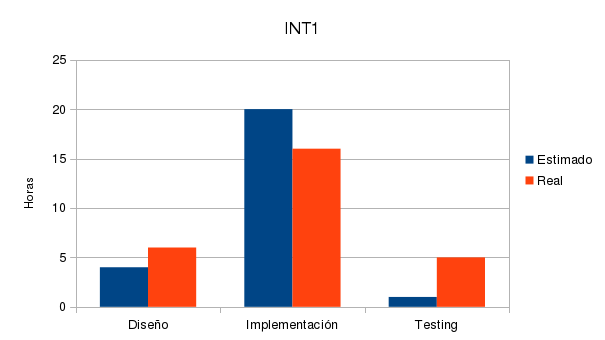
\includegraphics[width=0.53\textwidth]{img/Hint1.png}
    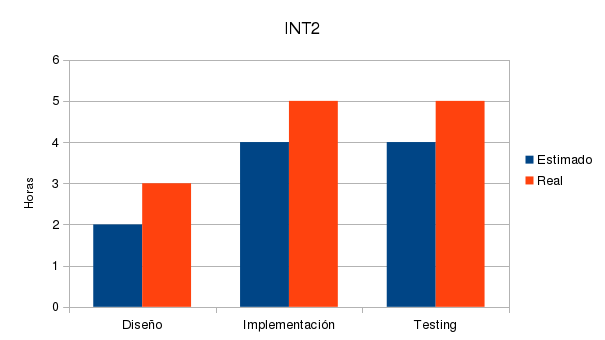
\includegraphics[width=0.53\textwidth]{img/Hint2.png}
    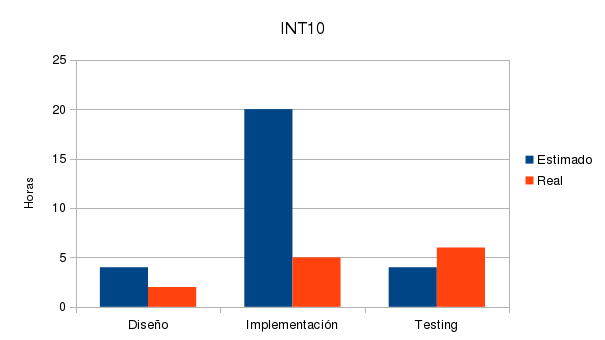
\includegraphics[width=0.53\textwidth]{img/Hint10.png}
    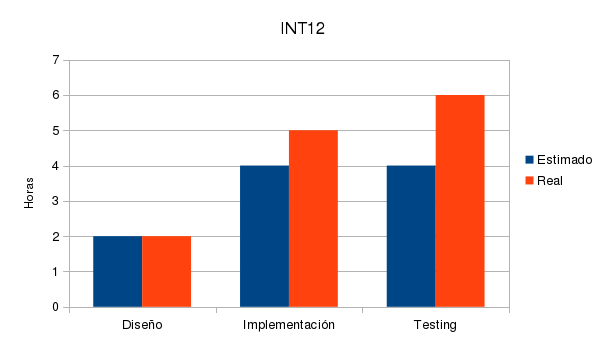
\includegraphics[width=0.53\textwidth]{img/Hint12.png}
    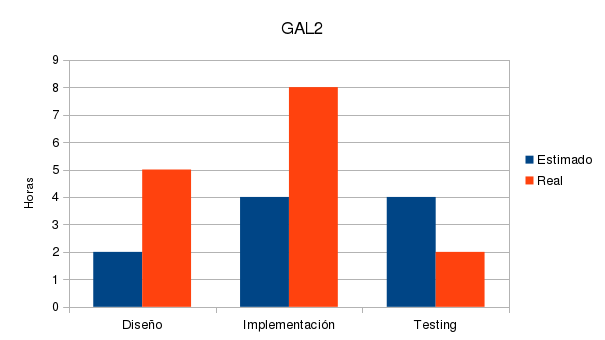
\includegraphics[width=0.53\textwidth]{img/Hgal2.png}
    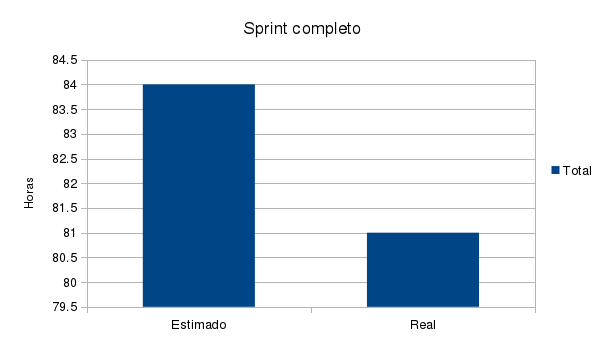
\includegraphics[width=0.53\textwidth]{img/Hsprint.png}


  \subsubsection{Avance del \textit{sprint} en funci\'on del tiempo}
  Aqu\'i se muestra como fue el progreso de las tareas a lo largo
  del tiempo. Podemos notar que comenzamos lento, por la cuesti\'on
  de no haber hecho un buen primer \textit{sprint}, pero al mejorarlo,
  logramos adaptarnos a la estimaci\'on.

  \vspace{1cm}

    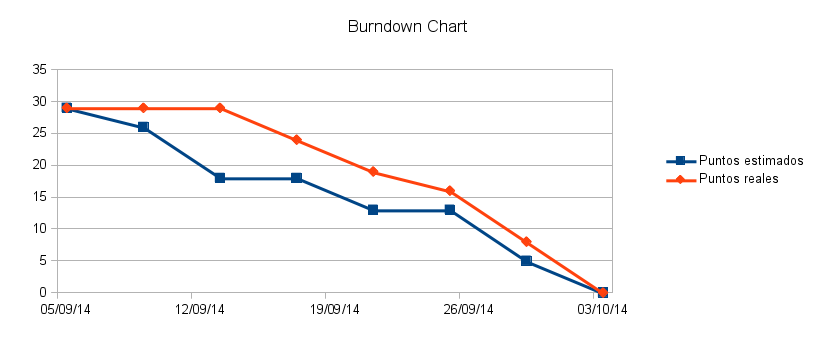
\includegraphics[width=0.8\textwidth]{img/burndownchart.png}

  TODO
  - agregar horas

%  \section{Dise\~no}
  \section{Dise\~no}

  \subsection{Diagrama de clases}

      \subsubsection{Abstracci\'on de los sensores}
          El enunciado habla sobre tres tipos de sensores bien concretos.
          Decidimos modelar a cada uno de ellos por separado. Es decir, no realizamos
          una abstracci\'on para Sensor. El motivo para sustentar esta decisi\'on
          que se refleja tanto a nivel de dise\~no como a nivel implementativo es
          el siguiente.

          Si bien los sensores se comportan de forma semejante,
          o mejor dicho, son polim\'orficos con respecto al mensaje \texttt{Sensar},
          no lo son vistos desde la perspectiva de un lenguaje est\'aticamente tipado.
          Esto es porque cada sensor devuelve un valor de un tipo o clase distinta.
          Una soluci\'on a esto hubiese sido no modelar los tipos de los valores de
          retorno con distintas clases, y poner \'unicamente un valor num\'erico
          (al estilo \textit{double}). Nos
          pareci\'o que perd\'iamos mucha sem\'antica con esta soluci\'on.

          Otra soluci\'on podr\'ia haber sido utilizar el patr\'on \textit{visitor} sobre
          un sensor abstracto, de manera que externamente se utilizara el sensor y se lo
          interpretara como la medici\'on apropiada. Esto nos pareci\'o que complejiza el
          modelo y la implementaci\'on innecesariamente, adem\'as de agregar acoplamiento
          entre funcionalidades claramente delimitadas.

          Al no haber realizado esta abstracci\'on se podr\'ia objetar que restringimos
          la extensibilidad en cuanto a m\'as o distinto tipo de sensores.
          Para responder a esta posible objeci\'on, debe observarse el modelado del
          \condiciones{}, el de los sensores y el del \arduino{}.
          Al desligar el sensor del \arduino{} conseguimos
          sensores vers\'atiles, en el sentido de que pueden depender de uno o varios sensores
          reales (es decir del mundo real). M\'as a\'un, los sensores modelados
          permiten tener l\'ogica interna para manejar los sensores del mundo real
          correctamente.

          Si se quisieran agregar nuevos tipos de sensores deber\'ian agregarse nuevas
          clases de sensores al modelo. Por supuesto deber\'a tambi\'en modificarse
          el c\'odigo de \condiciones{} para que se comunique
          con los nuevos sensores. Pero consideramos que esto es b\'asicamente inevitable,
          por m\'as que se realice una abstracci\'on del sensor, pues la l\'ogica
          de todo el sistema depender\'a, en este caso, de nuevos par\'ametros.

      \subsubsection{Abstracci\'on de los actuadores}
          Para el caso de los actuadores nos encontramos con una situaci\'on semejante
          a la reci\'en presentada. En este caso, sin embargo, optamos por realizar
          una abstracci\'on. Esta se denomina \texttt{Actuador Simple}. El nombre
          refleja la naturaleza sencilla de los actuadores modelados: b\'asicamente
          responden al mensaje \texttt{Suministrar} con una cantidad. Donde
          \texttt{Cantidad} es una clase que representa valores discretos y que adem\'as
          son interpretados por cada actuador de forma independiente.

          Esta abstracci\'on permite realizar una calibraci\'on de cada actuador a la
          hora de inicializar el sistema, que queda
          guardada en el actuador. Por otro lado permite, al \decisiones{},
          devolver decisiones en un formato semejante al almacenado en el
          \texttt{Plan Maestro} (y el descripto en el enunciado), que \'unicamente
          especifica cantidades aproximadas, las modeladas en la clase
          \texttt{Cantidades}.

      \subsubsection{Clase \texttt{Cantidad} y \calibrador{}}
          Justamente para que la cantidad tenga la sem\'antica apropiada en cada
          contexto, es necesario que el actuador sepa interpretarla.
          Para esto se lo debe calibrar al inicializar el sistema, de esto se
          encarga el \calibrador{}. Adem\'as la calibraci\'on podr\'ia ser incluida
          en el plan maestro para soportar distintos tipos de planta de forma
          c\'omoda. Si bien esto no estaba en el enunciado y no fue implementado,
          el modelo resulta extensible para estas modificaciones, ya que resulta
          esperable que se necesite este tipo de funcionalidad en el futuro.

      \subsubsection{Interacci\'on entre \decisiones{} y \condiciones{}}
          Inicialmente decidimos tener un \timer{} que peri\'odicamente llame a \condiciones{}
          con el mensaje \sensarCondiciones{}. Una vez recopilada la informaci\'on de los
          sensores, \condiciones{} mandaba el mensaje \tomarDecisiones{} a \decisiones{}.

          El problema con este protocolo es que \decisiones{} depende de \condiciones{}
          para entrar en juego. Por otro lado, \condiciones{} termina dependiendo de
          \condiciones{} a nivel dise\~no e implementaci\'on, lo cual no resulta razonable,
          pues son partes independientes del sistema y este acoplamiento puede ser evitado.

          Para esto usamos dos \timer{}. Los objetos que antes estaban acoplados, ahora
          pueden actuar libremente, siendo activados por \timer{}. \condiciones{}, luego
          de sensar, escribe los resultados en el \historial{}. \decisiones{} lee estos
          resultados al ser activado, y toma una decisi\'on.

          Otro aspecto interesante que surgi\'o al analizar esta interacci\'on es
          el comportamiento estilo \textit{observer} que se da entre \timer{} y
          \condiciones{} y entre \timer{} y \decisiones{}. Intentamos utilizar el patr\'on
          cl\'asico en el dise\~no, pero no result\'o natural. Los motivos son
          principalmente dos:
          \begin{itemize}
              \item El \timer{} se comporta como un observable, pero tiene una sutileza:
                  debe ajustarse el tiempo. Si bien esto puede ser solucionado de
                  forma prolija agregando objetos, decidimos que complicaba el dise\~no
                  por una cuesti\'on \'unicamente formal, que no facilitaba nada
                  concreto.
              \item Siempre que se siga usando al \timer{} como tal, el dise\~no seguir\'a
                  siendo extensible, en este aspecto. Pues la funcionalidad de \timer{}
                  no deber\'ia cambiar, por la esencia misma de un \timer{}.
          \end{itemize}
          Por estos motivos, creemeos que la extensibilidad no fue restringida al
          no utilizar un \textit{observer} cl\'asico.

      \subsubsection{\cliente{} y \servidor{}}
          Para que el sistema pueda funcionar al momento de implementarlo, nos result\'o esencial
          desacoplar totalmente el funcionamiento autom\'atico del mismo: manejo de
          actuadores, recopilar informaci\'on, tomar decisiones, etc. Del funcionamiento
          asincr\'onico debido al uso por parte del usuario: guardar entradas sobre la
          planta en el \historial{}, realizar consultas, etc.

          Para esto separamos el programa en dos procesos. El cliente y el servidor.
          Que a su vez, dieron lugar a dos objetos: \cliente{} y \servidor{}.

          El patr\'on utilizado es \textit{Fa\c{c}ade}. El \servidor{} es qui\'en
          encapsula todo el comportamiento autom\'atico del sistema.

          La comunicaci\'on con el cliente no es trivial, y se detalla su dise\~no a
          continuaci\'on.

          Para ver como se implement\'o la comunicaci\'on efectivamente, remitirse
          a la secci\'on de implementaci\'on.
          
      \subsubsection{Clase \mensaje{}}
          Al tener que transmitir los mensajes entre \cliente{} y \servidor{} entre
          procesos distintos, result\'o natural y conveniente especificar la forma
          y el prop\'osito de estos mensajes.
          Para esto utilizamos el patr\'on \textit{Command}. Esto da extensibilidad
          a la hora de agregar nuevas funcionalidades en \servidor{}, pues se pueden
          agregar nuevos comandos/mensajes comodamente.

          Como los procesos corriendo en un sistema operativo \textsc{UNIX} \'unicamente
          pueden comunicarse enviando \textit{bytes}, es decir, el sistema operativo no
          provee niveles de abstracci\'on para enviar objetos, la clase
          \constructorMensaje{} viene al caso. Y la abstracci\'on del \mensaje{}
          resulta muy \'util.
          El funcionamiento b\'asico es: para comunicarse el \cliente{} con el \servidor{}
          (y viceversa), el objeto crea un \mensaje{}.
          Luego, utilizando el m\'etodo \texttt{Serializar} de \mensaje{}, consigue un
          \textit{string} que representa al mensaje, y que env\'ia mediante un \textit{socket}.

          El objeto que recibe esto reconstruye el mensaje utilizando un \constructorMensaje{}
          y luego se env\'ia este mensaje.

          Si bien el proceso puede parecer complejo, es el \textit{tradeoff} m\'as simple
          \footnote{Que se nos ocurri\'o.} para que la soluci\'on no se salga del paradigma,
          pero al mismo tiempo, poder separar el cliente y el servidor en procesos distintos.

          Como se dijo arriba, remitirse a la secci\'on de implementaci\'on para ver
          los detalles de la comunicaci\'on, incluyendo c\'omo se ejecuta el mensaje
          una vez reconstruido por el servidor, mediante \textit{double dispatch}.

      \subsubsection{Clase \historial{}}
          El \historial{} tiene actualmente tres tipos de entradas, pero esto puede
          ser f\'acilmente modificado, gracias a utilizar herencia.
          La parte interesante del \historial{} es la forma en que es recorrido.
          Si bien esta funcionalidad no fue implementada si fue dise\~nada.
          Para recorrer el \historial{} se utiliza un \textit{Visitor}, en este caso
          representado por \recopilador{} quien sabe como recorrer \historial{}.

      \subsubsection{Dise\~no del \planmaestro{}}


  \subsection{Diagramas de objetos}
    En la secci\'on de diagramas se pueden observar dos diagramas de objetos.
    Uno detalla el estado del sistema haciendo omisi\'on de la parte que concierne
    al \historial{}.
    El segundo muestra el estado del \historial{} y algunos objetos pertinentes
    en un intervalo de unos pocos minutos de tiempo. Esto se debe a que el
    \historial{} almacena una gran cantidad de informaci\'on en poco tiempo.

  \subsection{Diagramas de secuencia}
    Los diagramas de secuencia muestran las dos acciones principales que
    representan el ciclo de vida del sistema.
    Una es una iteraci\'on del \decisiones{}, la otra, una iteraci\'on de \condiciones{}.

  TODO
  - pintar un mapita del diagrama de clases
    de acuerdo a las tareas del sprint
  - formatear e integrar los diagramas

%  \section{Implementaci\'on}
  \section{Implementaci\'on}
    \subsection{Testing}
      \paragraph{Para la integridad del \textit{software}}

        Para corroborar el correcto funcionamiento del sistema se crearon objetos para
        representar a los sensores y que simulararn a las mediciones.
        De forma an\'aloga se crearon objetos que simulen a los actuadores.
        
        Se utiliz\'o una \textit{suite} de tests para verificar que las
        serializarciones (en el caso de la comuncicaci\'on v\'ia \textit{sockets})
        y los mensajes y construcciones entre objetos fuesen compatibles.

      \paragraph{Para la \demostracion{}}
        Se probaron tanto instanciaciones de \arduino{} que devolvieran mediciones
        fijas como instanciaciones que devuelvan valores aleatorios o prefijados
        en archivos.
    \subsection{\textit{Script} de la \demostracion{}}

      En lo siguiente se pone a prueba el ciclo de vida b\'asico del sistema:
      despertar a los sensores y actuadores peri\'odicamente, tomar decisiones
      y guardar todo esto en el historial.

      Adem\'as se muestra c\'omo el usuario puede modificar el plan maestro, y,
      lo que es m\'as interesante, como el sistema actua conforme a este cambio.

      \begin{enumerate}
        \item Se corre el servidor (\texttt{./server}).
        \item El servidor carga el plan maestro.
        \item Se abre el cliente (\texttt{./client localhost}).
        \item Se le pide el estado fenol\'ogico a la planta y se
            agregan dos anotaciones.
            La respuesta es que la planta se encuentra en la etapa $4$, donde
            la humedad debe ser baja, el PH bajo y la temperatura baja.
        \item El \timer{} de \condiciones{} se activa varias veces. As\'i se guardan las
            mediciones de los sensores y de la central meteorol\'ogica.
            Se observan los valores: PH bajo, Humerdad bajo, Temperatura baja y
            Probabilidad de lluvia $10\%$.
            Todo esto se guarda en el historial.
        \item Luego de algunos sensados se activa el \timer{} de \decisiones{}\footnote{
            los tiempos son $1m$ para el de \condiciones{} y $5m$ para el de \decisiones{}.}.
        \item \decisiones{} consulta el \'ultimo sensado en el historial y pregunta al plan
            maestro la estapa actual.
        \item Dados estos valores decide una cantidad para cada actuador: poco, poco, poco, nada.
        \item Env\'ia la decisi\'on a \manejadorAct{}.
        \item \manejadorAct{} se comunica con los actuadores indicando la cantidad
            correspondiente.
        \item Cada actuador se comunica con su arduino indicando el nuevo valor de su
            \textit{dimmer}.
        \item El tomador de decisiones guarda la decisi\'on tomada en el historial.
        \item Se realiza una nueva ronda de sensados.
        \item El usuario pide al cliente modificar el plan maestro.
        \item Se modifica el estado $4$ del plan. Ahora la humedad debe ser abundante,
            \textbf{el PH bajo} y la temperatura baja.
        \item Se muestra en pantalla, del servidor, que se modific\'o el plan.
        \item Luego de otro sensado se activa nuevamente el \timer{} de \decisiones{}.
        \item Se prosigue de forma an\'aloga pero administrando una cantidad
            \textbf{distinta} pues el plan es distinto.
      \end{enumerate}

    \subsection{Comunicaci\'on por \textit{Sockets}}
      La comunicaci\'on entre cliente y servidor se realiza utilizando \textsc{UNIX}
      \textit{sockets}.
      Cuando se crea el objeto servidor, se configura un \textit{file descriptor} con
      un \textit{socket} \textit{bindeado} a la primera IP no-local que se encuentre.
      El servidor se pone en modo escucha, esperando una conexi\'on \textsc{TCP}
      al puerto configurado. Al finalizar la conexi\'on el servidor se vuelve a poner
      en modo escucha.
      Es importante notar que por m\'as que el servidor est\'e esperando mensajes,
      simultaneamente, funcionan todos los eventos asicr\'onicos de timers, con lo cual,
      ambas funcionalidades est\'an desacopladas.

      Por la contraparte, la atenci\'on de la comunicaci\'on funciona de la siguiente manera.
      El servidor espera mensajes a traves del \textit{file descriptor} mencionado antes.
      Cuando recibe una cadena de texto (que es lo unico que puede enviarse a traves de
      \textit{sockets}) se la env\'ia a \constructorMensaje{} que se encarga de
      parsear y reconstruir el mensaje original.
      Una vez reconstruido, el servidor ejecuta el mensaje, pasandose a si mismo como par\'ametro.
      Mediante este \textit{double dispatch} el mensaje sabe que debe ejecutar cierta funcionaldidad
      y devolver un mensaje de respuesta. El servidor entonces env\'ia este mensaje serializado
      de vuelta al cliente. El mensaje de respuesta se maneja con un mecanismo an\'alogo.


%      \subsubsection{Bootstrapping}
%      FALTA


%  \section{Retrospectiva}
  \section{Retrospectiva}

  \subsection{Asunciones}
    \subsubsection{Fenolog\'ia}
      Por falta de conocimiento en el \'area asumimos que los estad\'ios de maduraci\'on
      de la planta estaban determinados por lapsos fijos de tiempo. Esto quiere decir que
      el paso de una etapa a la otra est\'a solo controlado por el paso de los meses. 
      Esto provoca que el ingreso de indicadores fenol\'ogicos por parte del usuario
      sea meramente informativo.  

  \subsection{Inconvenientes encontrados}
    \subsubsection{Tareas programadas en el \sprintback{}}
      Al momento de definir las tareas no ten\'iamos experiencia en separar y definir
      tareas concretas para un proyecto. A pesar de nuestro intento por modularizar
      las tareas y no olvidar partes esenciales result\'o que b\'asicamente obviamos
      las tareas de modelado y dise\~no. Por otro lado, las tareas de implementaci\'on
      resultaron modularizadas de forma poco conveniente, pues no se correspond\'ian
      con las clases, que fueron dise\~nadas luego. Si bi\'en el \sprintback{} tuvo
      este inconveniente, a la hora de ponernos a trabajar notamos r\'apidamente
      el problema, y logramos distribuirnos las tareas de forma eficiente.
    \subsubsection{Horas estimadas de implementaci\'on}
      Luego de haber ajustado las tareas del \sprintback{} logramos una buena
      estimaci\'on de las horas de dise\~no, pues habiamos experimentado cuanto
      nos pod\'ia tomar. Por otro lado las horas de implementaci\'on quedaron un tanto
      ajustadas, si bien la diferencia con las horas reales de implementaci\'on no
      fue tan grande.

    \subsection{Pr\'oxima iteraci\'on -- no implementado}
      \subsubsection{Decisiones dependientes del \textit{input} del usuario}
        En lo que se implement\'o las decisiones de como actuar dependen del plan
        maestro, y de los datos recolectados por los sensores.
        Las caracter\'isticas escritas por el usuario sirven a modo de \textit{log}
        para que el usuario pueda chequear la evoluci\'on de la planta.

        En una nueva iteraci\'on se podr\'ia modificar el proceso de decisi\'on para
        que tome en cuenta las caracter\'isticas escritas por el usuario en el
        historial.

        Para esto deber\'ia agregarse un nuevo tipo de entrada en el historial
        que permita guardar caracter\'isticas bien definidas con un formato apropiado.

        Para agregar esto al dise\~no bastar\'a heredar un nuevo tipo de entrada
        del historial, y que \decisiones{} use esta nueva clase.

      \subsubsection{SMS}

      \subsubsection{Recopilador}
        Servidor deberia habar con recopilador


  TODO
  - proxima iteracion

\end{document}
